% ===============================================================
% APRESENTAÇÃO FINAL - TCC2 - SENAC SANTO AMARO
% ===============================================================
% Baseada no template do curso e no estilo da apresentacao_previa.tex.
% Duração: 30 minutos (~1 a 1,5 min por slide de conteúdo).
%   Problema ............ ~3 min   (slides 3-4)
%   Objetivos e método .. ~5 min   (slides 5-8)
%   Desenvolvimento ..... ~7 min   (slides 9-14)
%   Resultados .......... ~11 min  (slides 15-23)
%   Conclusão ........... ~4 min   (slides 24-26)
% Os slides do apêndice são de apoio para a arguição da banca.
%
% Todos os números vêm do documento escrito (tcc2.tex), seção de
% Resultados, e do repositório Codigo-do-TCC2. Os gráficos de corrente
% usam sections/dados/*.dat (gerados por
% medicoes/exportar_ciclo_corrente.py, comandos no docstring).
%
% Compilar a partir da pasta tcc2/:
%   pdflatex apresentacao_tcc2.tex   (2x)
% ===============================================================

\documentclass[
    aspectratio=169,
    12pt,
    brazil
]{beamer}

% ---------------------------------------------------------------
% PACOTES
% ---------------------------------------------------------------
\usepackage[T1]{fontenc}
\usepackage[utf8]{inputenc}
\usepackage[brazil]{babel}
\usepackage{graphicx}
\usepackage{booktabs}
\usepackage{array}
\usepackage{tikz}
\usetikzlibrary{arrows.meta,positioning,fit,calc}
\usepackage{pgfplots}
\pgfplotsset{compat=1.18}
\usepgfplotslibrary{groupplots}
\usepackage{appendixnumberbeamer}

% ---------------------------------------------------------------
% TEMA E CORES (template do curso)
% ---------------------------------------------------------------
\usetheme{default}
\useinnertheme{circles}
\setbeamertemplate{navigation symbols}{}

\definecolor{senacblue}{RGB}{0,51,102}
\definecolor{senacorange}{RGB}{243,146,0}

\setbeamercolor{structure}{fg=senacblue}
\setbeamercolor{frametitle}{fg=white,bg=senacblue}
\setbeamercolor{title}{fg=senacblue}
\setbeamercolor{section in toc}{fg=senacblue}
\setbeamercolor{itemize item}{fg=senacorange}
\setbeamercolor{itemize subitem}{fg=senacorange}
\setbeamerfont{frametitle}{series=\bfseries}
\setbeamertemplate{frametitle}[default][left]

\setbeamertemplate{footline}{%
  \leavevmode%
  \hbox{%
    \begin{beamercolorbox}[wd=.34\paperwidth,ht=2.4ex,dp=1ex,leftskip=1em]{author in head/foot}%
      \usebeamerfont{author in head/foot}\insertshortauthor
    \end{beamercolorbox}%
    \begin{beamercolorbox}[wd=.5\paperwidth,ht=2.4ex,dp=1ex,center]{title in head/foot}%
      \usebeamerfont{title in head/foot}\insertshorttitle
    \end{beamercolorbox}%
    \begin{beamercolorbox}[wd=.16\paperwidth,ht=2.4ex,dp=1ex,rightskip=1em]{title in head/foot}%
      \usebeamerfont{title in head/foot}\hfill\insertframenumber/\inserttotalframenumber
    \end{beamercolorbox}%
  }\vskip0pt%
}
\setbeamercolor{author in head/foot}{bg=senacblue,fg=white}
\setbeamercolor{title in head/foot}{bg=senacblue!85,fg=white}

% ---------------------------------------------------------------
% LOGO DO SENAC (grande na capa, pequena no canto dos demais slides)
% ---------------------------------------------------------------
\newcommand{\logosenacgrande}{%
  \IfFileExists{assets/logo-senac.png}{%
    
\includegraphics[height=2.2cm]{assets/logo-senac.png}%
  }{\fbox{\bfseries\color{senacblue}SENAC}}%
}
\newcommand{\logosenacpequena}{%
  \IfFileExists{assets/logo-senac.png}{%
    
\includegraphics[height=0.8cm]{assets/logo-senac.png}%
  }{\fbox{\scriptsize\bfseries\color{senacblue}SENAC}}%
}
\addtobeamertemplate{frametitle}{}{%
  \begin{tikzpicture}[remember picture,overlay]
    \node[anchor=north east,fill=white,rounded corners=2pt,inner sep=3pt]
      at ([xshift=-6pt,yshift=-5pt]current page.north east) {\logosenacpequena};
  \end{tikzpicture}%
}

% ---------------------------------------------------------------
% CORES DOS FLUXOS (as mesmas do documento escrito)
% ---------------------------------------------------------------
\definecolor{corNuvem}{HTML}{2A78D6}
\definecolor{corBorda}{HTML}{EB6834}
\definecolor{corGrade}{HTML}{E1E0D9}
\definecolor{corEixo}{HTML}{898781}
\definecolor{corOk}{HTML}{008300}
\definecolor{corFalha}{HTML}{C62828}

\pgfplotsset{
    estiloSlides/.style={
        grid=major, grid style={color=corGrade, line width=0.3pt},
        axis x line*=bottom, axis y line*=left,
        axis line style={color=corEixo}, tick style={color=corEixo},
        tick label style={font=\scriptsize}, label style={font=\scriptsize},
        title style={font=\footnotesize\bfseries},
        legend style={font=\scriptsize, draw=none, fill=none},
        legend cell align=left,
        /pgf/number format/use comma, /pgf/number format/1000 sep={.},
    },
}

% Número grande + legenda curta
\newcommand{\bignum}[3][senacblue]{%
  \begin{minipage}[t]{\linewidth}\centering
    {\fontsize{24}{26}\selectfont\bfseries\color{#1}#2\par}
    \vspace{2pt}
    {\scriptsize\color{black!70}#3\par}
  \end{minipage}}

% Etiqueta pequena de status
\newcommand{\etiqueta}[2]{\tikz[baseline=(t.base)]\node[fill=#1,text=white,rounded corners=2pt,
  inner sep=2pt,font=\tiny\bfseries](t){#2};}

% Nota de rodapé do slide (fonte dos dados)
\newcommand{\fonteslide}[1]{\par\vfill{\tiny\color{black!60}#1\par}}

% ---------------------------------------------------------------
% DADOS DA APRESENTAÇÃO
% ---------------------------------------------------------------
\title[OCR em borda × nuvem em \textit{smart metering}]{Análise comparativa de desempenho e eficiência energética entre processamento de OCR em borda e em nuvem aplicado à \textit{smart metering}}
\subtitle{Apresentação final --- TCC2}
\author[Marcelo, Gustavo e Christian]{Marcelo Fernandes de Oliveira Junior\\Gustavo Oliveira dos Santos\\Christian Lima Santana}
\institute[SENAC Santo Amaro]{%
  SENAC - Unidade Santo Amaro\\
  Bacharelado em Ciência da Computação\\
  \footnotesize Orientador: Prof. Afonso César Lelis Brandão}
\date{São Paulo, 2026}

% ===============================================================
\begin{document}

% ---------------------------------------------------------------
% CAPA
% ---------------------------------------------------------------
{
\setbeamertemplate{footline}{}
\begin{frame}[plain]
  \centering
  \vspace{-0.2cm}
  \logosenacgrande

  \vspace{0.2cm}
  \begin{minipage}{0.86\textwidth}\centering
  {\usebeamerfont{title}\usebeamercolor[fg]{title}\bfseries\normalsize\inserttitle\par}
  \end{minipage}
  \vspace{0.1cm}
  {\small\insertsubtitle\par}

  \vspace{0.25cm}
  {\footnotesize\insertauthor\par}
  \vspace{0.12cm}
  {\scriptsize\insertinstitute\par}
  \vspace{0.12cm}
  {\scriptsize\insertdate\par}
\end{frame}
}

\begin{frame}{Roteiro}
  \tableofcontents
\end{frame}

% ===============================================================
\section{Problema}
% ===============================================================
\begin{frame}{Contexto}
  \begin{columns}[c]
    \column{0.55\textwidth}
    \begin{itemize}\small
      \setlength{\itemsep}{4pt}
      \item Trocar medidores analógicos por inteligentes tem alto custo inicial, o principal entrave à adoção em larga escala.
      \item \textbf{\textit{Retrofitting}}: uma câmera barata lê o mostrador que já existe.
      \item \textbf{LoRaWAN}: longo alcance e baixo consumo, mas \textbf{pouca banda} (até 222~bytes por pacote em DR6).
      \item Onde fazer o \textbf{OCR}? No próprio nó (\textcolor{corBorda}{\textbf{borda}}) ou em um servidor (\textcolor{corNuvem}{\textbf{nuvem}}).
    \end{itemize}
    \column{0.42\textwidth}
    \centering
    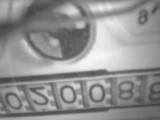
\includegraphics[width=0.85\linewidth]{assets/apresentacao/bancada_quadro.jpg}\\[2pt]
    {\tiny O hidrômetro da bancada visto pela câmera do nó: quadro de $160 \times 120$ pixels em tons de cinza}
  \end{columns}
\end{frame}

\begin{frame}[fragile]{Problema e \textit{trade-off}}
  \centering
  \begin{tikzpicture}[
      caixa/.style={draw=#1, rounded corners=4pt, fill=#1!8, inner sep=6pt, font=\footnotesize}]
    \node[caixa=corBorda] (b) at (0,0) {\begin{minipage}[t][2.75cm][t]{5.6cm}\raggedright
      {\bfseries\color{corBorda}Borda}\\[3pt]
      + transmite só a leitura (poucos bytes)\\
      -- inferência em um microcontrolador\\
      -- modelo limitado pela memória (4~MB de PSRAM)\end{minipage}};
    \node[caixa=corNuvem] (n) at (6.6,0) {\begin{minipage}[t][2.75cm][t]{5.6cm}\raggedright
      {\bfseries\color{corNuvem}Nuvem}\\[3pt]
      + inferência rápida, modelo sem restrição\\
      + atualização só no servidor\\
      -- transmite a imagem inteira, em vários pacotes\end{minipage}};
  \end{tikzpicture}

  \vspace{0.45cm}
  \begin{block}{Pergunta de pesquisa}
    \small Como a adoção do processamento em borda ou em nuvem impacta a eficiência energética,
    a acurácia, a complexidade de desenvolvimento de firmware e o desempenho computacional de um
    sistema IoT de leitura de medidores analógicos?
  \end{block}
\end{frame}

% ===============================================================
\section{Objetivos e método}
% ===============================================================
\begin{frame}{Objetivos}
  \begin{block}{Objetivo geral}
    \small Comparar a viabilidade técnica, a acurácia e o consumo energético entre o OCR feito
    \textbf{no ESP32-CAM} (borda) e \textbf{em um servidor} (nuvem), usando LoRaWAN como meio de
    transmissão.
  \end{block}
  \vspace{0.1cm}
  {\small\bfseries\color{senacblue}Objetivos específicos}
  \vspace{0.05cm}
  \small
  \renewcommand{\arraystretch}{1.25}
  \begin{tabular}{@{}r >{\raggedright\arraybackslash}p{12.6cm}@{}}
    \textbf{\color{senacorange}1} & Implementar os dois fluxos: OCR no nó e envio da imagem para o servidor. \\
    \textbf{\color{senacorange}2} & Configurar o enlace LoRaWAN no plano AU915, conforme o Ato n\textordmasculine~14.448 da ANATEL, e o repouso do nó entre leituras, reduzindo o consumo (corrente em repouso, mA). \\
    \textbf{\color{senacorange}3} & Comparar os fluxos em acurácia (\%), latência, energia por leitura (mAh) e volume de dados (bytes). \\
  \end{tabular}
\end{frame}

\begin{frame}{Hipóteses}
  \centering
  \begin{tikzpicture}[
      cartao/.style={draw=senacblue, rounded corners=4pt, fill=senacblue!5, inner sep=6pt,
                     anchor=north}]
    \node[cartao] at (0,0) {\begin{minipage}[t][4.15cm][t]{4.1cm}\raggedright
      {\large\bfseries\color{senacorange}H1}\\[3pt]
      {\footnotesize A quantização em INT8, aplicada ao classificador usado nos dois fluxos, causa redução de acurácia em comparação com a versão em ponto flutuante de 32 bits do mesmo modelo.}\end{minipage}};
    \node[cartao] at (4.85,0) {\begin{minipage}[t][4.15cm][t]{4.1cm}\raggedright
      {\large\bfseries\color{senacorange}H2}\\[3pt]
      {\footnotesize O processamento local apresenta custo computacional maior, no dispositivo final, em comparação com o processamento remoto.}\end{minipage}};
    \node[cartao] at (9.7,0) {\begin{minipage}[t][4.15cm][t]{4.1cm}\raggedright
      {\large\bfseries\color{senacorange}H3}\\[3pt]
      {\footnotesize O processamento em nuvem apresenta autonomia energética inferior durante a transmissão de mensagens, em comparação com o processamento local.}\end{minipage}};
  \end{tikzpicture}

  \vspace{0.3cm}
  {\scriptsize\color{black!70}Latência e entrega dos dados foram medidas de forma complementar.}
\end{frame}

\begin{frame}{Como cada hipótese é testada}
  \centering
  \footnotesize
  \renewcommand{\arraystretch}{1.35}
  \begin{tabular}{@{}l >{\raggedright\arraybackslash}p{4.3cm} >{\raggedright\arraybackslash}p{6.6cm}@{}}
    \toprule
    & \textbf{Métricas} & \textbf{Como foi medido} \\
    \midrule
    \textbf{\color{senacorange}H1} & Acurácia por dígito, F1, leitura exata
      & Mesmo classificador em float32 e INT8: 7.378 recortes de validação e 30 fotos do hidrômetro físico; teste pareado de McNemar \\
    \textbf{\color{senacorange}H2} & Tempo de processamento, uso de CPU, frequência, pico de PSRAM
      & No próprio nó: firmware de depuração (61 capturas) e firmwares instrumentados (30 ciclos por fluxo) \\
    \textbf{\color{senacorange}H3} & Carga por leitura (mAh) e autonomia
      & INA219 a 100 amostras/s em cerca de 30 ciclos por fluxo; autonomia por modelo para uma bateria de 2.000~mAh \\
    \textit{Compl.} & Latência e entrega
      & Do despertar do nó até o dado no servidor; entrega por pacote e por leitura (Fisher) \\
    \bottomrule
  \end{tabular}
\end{frame}

\begin{frame}{Método}
  \centering
  \begin{tikzpicture}[
      font=\footnotesize,
      etapa/.style={draw=senacblue, rounded corners=3pt, fill=senacblue!8, align=center,
                    minimum height=1.4cm, text width=2.1cm},
      seta/.style={-{Stealth[length=2mm]}, thick, senacblue}]
    \node[etapa] (a) {\textbf{1}\\Pesquisa bibliográfica (ST01 a ST09)};
    \node[etapa, right=0.3cm of a] (b) {\textbf{2}\\Treinar e quantizar o OCR};
    \node[etapa, right=0.3cm of b] (c) {\textbf{3}\\Implementar os dois fluxos};
    \node[etapa, right=0.3cm of c] (d) {\textbf{4}\\Medir em bancada, $\approx$30 leituras};
    \node[etapa, right=0.3cm of d] (e) {\textbf{5}\\Comparar com testes estatísticos};
    \draw[seta] (a) -- (b); \draw[seta] (b) -- (c); \draw[seta] (c) -- (d); \draw[seta] (d) -- (e);
  \end{tikzpicture}

  \vspace{0.6cm}
  \begin{block}{Princípio do experimento}
    \small Mesmo hardware, mesmos modelos INT8 e mesmo enlace nos dois fluxos: a única variável é
    \textbf{onde} o OCR é executado.
  \end{block}
\end{frame}

% ===============================================================
\section{Desenvolvimento}
% ===============================================================
\begin{frame}{Hardware}
  \begin{columns}[c]
    \column{0.56\textwidth}
    \centering
    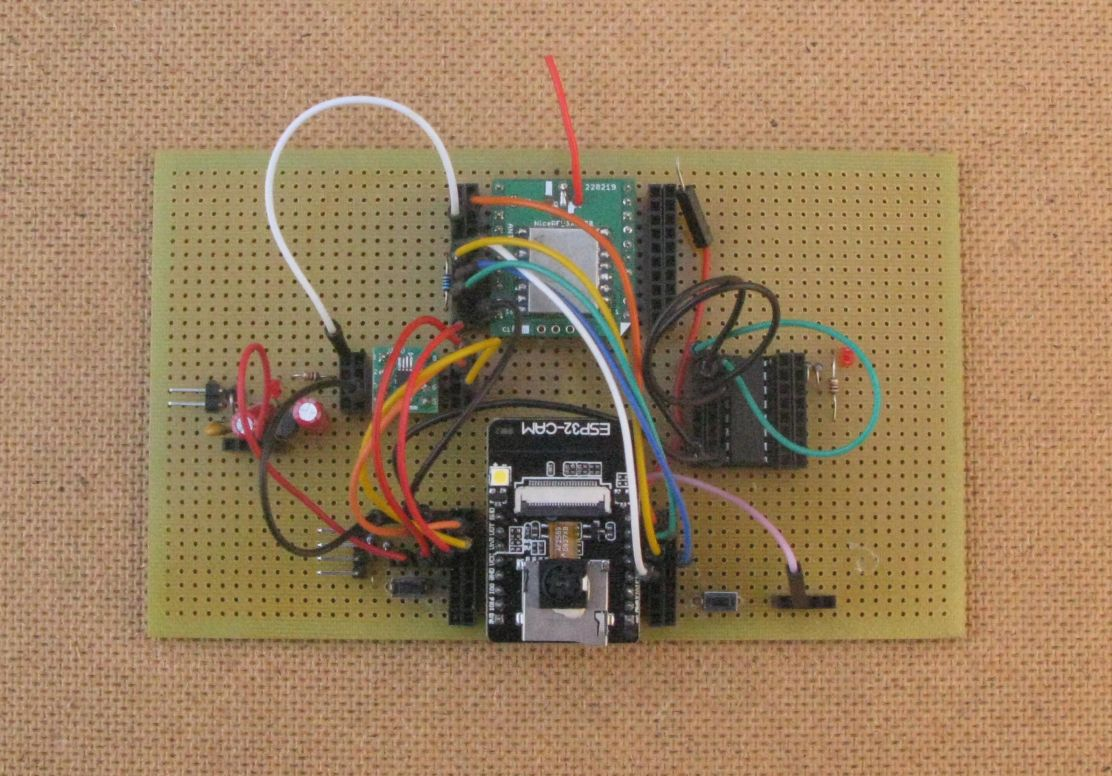
\includegraphics[width=\linewidth]{sections/imagens/ESP32CAM_LoRa.jpg}\\[1pt]
    {\tiny Nó sensor: ESP32-CAM + Radioenge RD49C}
    \column{0.42\textwidth}
    \begin{itemize}\small
      \item \textbf{ESP32-CAM}: câmera, OCR e controle (240~MHz, 4~MB de PSRAM)
      \item \textbf{Radioenge RD49C}: rádio LoRaWAN por comandos AT
      \item \textbf{Heltec LoRa32}: receptor de canal único em 915,9~MHz
      \item \textbf{Arduino + INA219}: corrente do nó a 100~Hz
    \end{itemize}
  \end{columns}
\end{frame}

\begin{frame}[fragile]{Arquitetura dos dois fluxos}
  \centering
  \resizebox{0.72\textwidth}{!}{%
    \begin{tikzpicture}[
        font=\tiny,
        node distance=3.5mm and 3.5mm,
        bloco/.style={draw, rounded corners=2pt, align=center, fill=white,
                     minimum height=6mm, text width=#1},
        bloco/.default=4.8cm,
        seta/.style={-{Stealth[length=1.5mm]}, thick},
        rotulo/.style={font=\tiny\itshape, align=center}
    ]
        \node[bloco] (hidro) {Hidrômetro analógico (mostrador de roletes)};
        \node[bloco, below=of hidro] (cam)
            {\textbf{ESP32-CAM}\\captura um quadro $160\times120$ em tons de cinza e dorme entre leituras};
        \node[bloco=4.2cm, draw=corBorda, below left=5mm and -1.5cm of cam] (borda)
            {\textbf{\color{corBorda}Fluxo em borda}\\classifica os 6 dígitos na ROI calibrada\\envia a leitura: \textbf{9 bytes, 1 pacote}};
        \node[bloco=4.2cm, draw=corNuvem, below right=5mm and -1.5cm of cam] (nuvem)
            {\textbf{\color{corNuvem}Fluxo em nuvem}\\comprime em JPEG (qualidade 90)\\envia a imagem: \textbf{$\approx$4~KB em blocos de 181 bytes}};
        \node[bloco] (radio) at ($(borda.south)!0.5!(nuvem.south)+(0,-8mm)$)
            {\textbf{Radioenge RD49C}\\LoRaWAN por UART (comandos AT), classe A};
        \node[draw, dashed, rounded corners=3pt, inner sep=1.8mm,
              fit=(cam) (borda) (nuvem) (radio),
              label={[font=\tiny\bfseries, anchor=north west]north west:Nó sensor}] {};
        \node[bloco, below=7mm of radio] (rx)
            {\textbf{Receptor LoRa32}\\escuta o canal de 915,9~MHz e repassa os quadros recebidos};
        \node[bloco, below=of rx] (pc)
            {\textbf{Servidor}\\descriptografa; lê a leitura (FPort 2) ou remonta o JPEG e executa o OCR (FPort 1)};
        \draw[seta] (hidro) -- (cam);
        \draw[seta] (cam.south) -- ++(0,-1.5mm) -| (borda.north);
        \draw[seta] (cam.south) -- ++(0,-1.5mm) -| (nuvem.north);
        \draw[thick] (borda.south) |- ([yshift=2.5mm]radio.north);
        \draw[thick] (nuvem.south) |- ([yshift=2.5mm]radio.north);
        \draw[seta] ([yshift=2.5mm]radio.north) -- (radio.north);
        \draw[seta] (radio) -- node[rotulo, right=1mm]
            {AU915, DR6 (SF8 / 500~kHz), canal fixo, ABP} (rx);
        \draw[seta] (rx) -- node[rotulo, right=1mm] {USB-serial} (pc);
    \end{tikzpicture}%
  }
\end{frame}

\begin{frame}{Enlace LoRaWAN}
  \begin{columns}[t]
    \column{0.5\textwidth}
    {\small\bfseries\color{senacblue}Configuração}
    \begin{itemize}\small
      \item AU915, \textbf{DR6}: SF8 com 500~kHz, canal fixo de 915,9~MHz.
      \item Item 10.3 do Ato n\textordmasculine~14.448 (largura $\geq$ 500~kHz): dispensa o salto de frequência.
      \item Ativação ABP, sem confirmação e sem \textit{downlink}.
      \item Módulo em \textbf{classe A}: desliga o rádio fora das janelas de recepção.
    \end{itemize}
    \column{0.47\textwidth}
    {\small\bfseries\color{senacblue}Mensagens}
    \begin{itemize}\small
      \item \textcolor{corBorda}{\textbf{Borda}}: id + estado + 6 dígitos ASCII = \textbf{9 bytes}.
      \item \textcolor{corNuvem}{\textbf{Nuvem}}: blocos de 175 bytes de JPEG + 6 de cabeçalho (id, índice, total) = \textbf{181 bytes} (máximo em DR6: 222).
      \item Intervalo de 7~s entre blocos (escolha conservadora).
      \item Cerca de \textbf{450 vezes menos dados} por leitura na borda.
    \end{itemize}
  \end{columns}
\end{frame}

\begin{frame}{Modelos: da U-Net + CRNN à CNN simples}
  \begin{columns}[t]
    \column{0.48\textwidth}
    {\small\bfseries\color{senacblue}U-Net + CRNN + CTC}
    \begin{itemize}\small
      \item Em computador: 86,67\% das sequências completas (26/30).
      \item No nó: a U-Net pedia uma \textit{arena} de \textbf{15,3~MB} (há 4~MB de PSRAM).
      \item O CTC usa \texttt{REDUCE\_PROD}, ausente no TensorFlow Lite Micro do \textit{core}.
    \end{itemize}
    \etiqueta{corFalha}{DESCARTADO NO NÓ}
    \column{0.48\textwidth}
    {\small\bfseries\color{senacblue}CNN simples (adotado)}
    \begin{itemize}\small
      \item Localização da janela ($192 \times 192$) e classificador de um dígito ($28 \times 28$).
      \item Treino com 49.038 recortes públicos + 24 do ESP32-CAM (ajuste fino).
      \item Quantização INT8 pós-treino: os dois modelos somam \textbf{93,3~KB}.
    \end{itemize}
    \etiqueta{corOk}{EXECUTA NOS DOIS FLUXOS}
  \end{columns}
\end{frame}

\begin{frame}{Leitura no nó: ROI calibrada e face da roda}
  \begin{columns}[c]
    \column{0.42\textwidth}
    \centering
    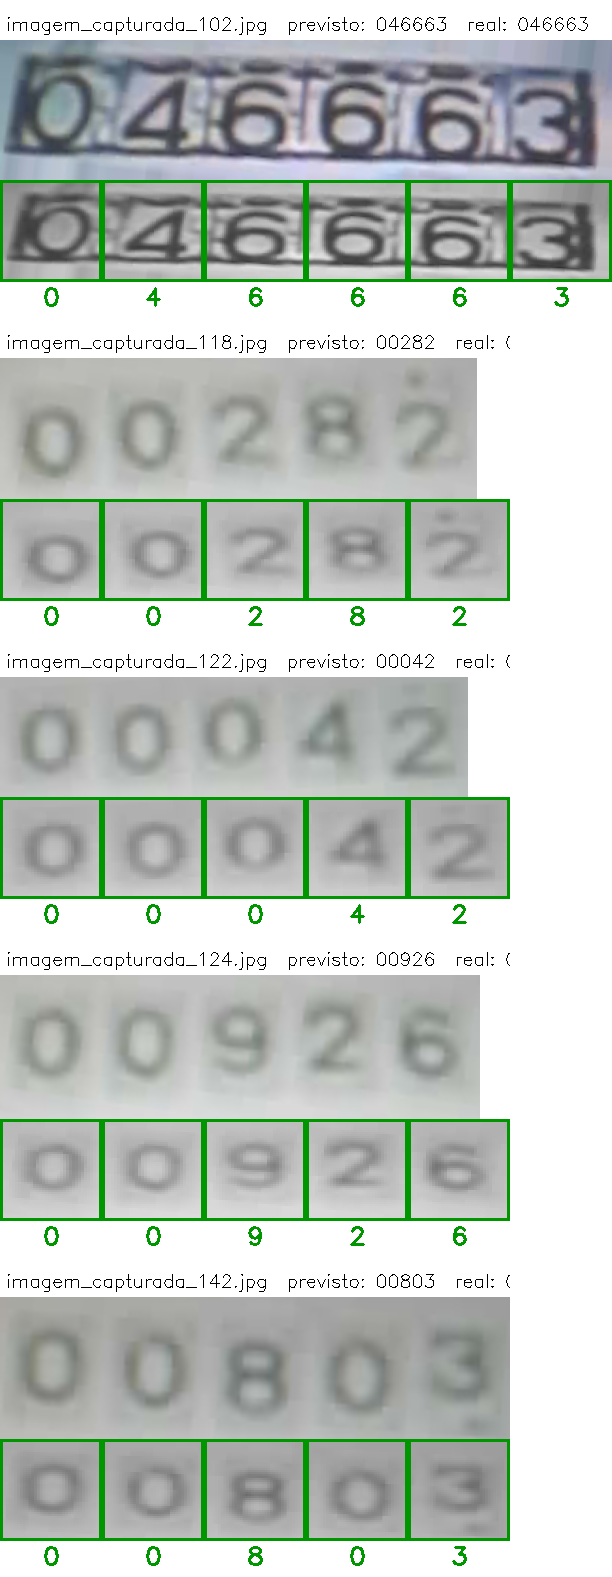
\includegraphics[width=0.9\linewidth,trim=0 1265 0 0,clip]{sections/imagens/ocr_leitura_caixa_manual.png}\\[2pt]
    {\tiny Janela dos dígitos, fatias e leitura prevista}
    \column{0.55\textwidth}
    \begin{itemize}\small
      \setlength{\itemsep}{3pt}
      \item A localização automática \textbf{falhou} em medidores reais (próximo slide).
      \item Câmera fixa: a janela (\textbf{ROI}) é calibrada uma vez, na instalação, e gravada na memória do nó.
      \item Cada fatia é cortada na \textbf{face da roda} (14\% a 74\% da largura) e classificada.
      \item Mesmo código e mesmos pixels na placa e no servidor: leituras iguais em \textbf{33 de 33} quadros.
    \end{itemize}
  \end{columns}
\end{frame}

% ===============================================================
\section{Resultados}
% ===============================================================
\begin{frame}{H1 - Quantização INT8}
  \begin{columns}[c]
    \column{0.52\textwidth}
    \centering
    \begin{tikzpicture}
      \begin{axis}[estiloSlides, ybar, width=\linewidth, height=5.2cm,
          bar width=1.1cm, ymin=90, ymax=97, enlarge x limits=0.6,
          symbolic x coords={Float32,INT8}, xtick=data,
          ylabel={Acurácia por dígito (\%)},
          nodes near coords, nodes near coords style={font=\footnotesize\bfseries},
          point meta=explicit symbolic]
        \addplot[fill=senacblue!70, draw=none] coordinates {(Float32,95.46) [95,46] (INT8,95.38) [95,38]};
      \end{axis}
    \end{tikzpicture}\\
    {\tiny 7.378 recortes de validação}
    \column{0.45\textwidth}
    \begin{itemize}\small
      \item Diferença de \textbf{6 recortes} (0,08 p.p.)
      \item McNemar: $p = 0{,}29$ (14 contra 8 discordantes)
      \item Macro-F1: 0,946 contra 0,945
      \item Hidrômetro físico: \textbf{25/30} leituras nas duas versões ($p = 1{,}0$)
    \end{itemize}
    \vspace{0.15cm}
    \etiqueta{senacorange}{CONFIRMADA NO SENTIDO}\\[2pt]
    {\scriptsize mas a redução é desprezível}
  \end{columns}
\end{frame}

\begin{frame}{Leitura de ponta a ponta: o gargalo é a janela}
  \begin{columns}[c]
    \column{0.6\textwidth}
    \centering
    \begin{tikzpicture}
      \begin{axis}[estiloSlides, xbar, scale only axis, width=4.4cm, height=4.2cm,
          bar width=0.42cm, xmin=0, xmax=112, xtick={0,20,40,60,80,100}, enlarge y limits=0.14,
          symbolic y coords={fis,man2,man,prev}, ytick={fis,man2,man,prev},
          yticklabels={{Físico: ROI + face},{Comum: à mão, endireitada},{Comum: marcada à mão},{Comum: prevista}},
          y dir=reverse, yticklabel style={font=\tiny, align=right},
          xlabel={Leituras exatas (\%)},
          nodes near coords, nodes near coords style={font=\scriptsize\bfseries, anchor=west},
          point meta=explicit symbolic]
        \addplot[fill=senacblue!70, draw=none, bar shift=0pt]
          coordinates {(0,prev) [0\%] (46,man) [46\%] (82,man2) [82\%] (83,fis) [83\%]};
      \end{axis}
    \end{tikzpicture}
    \column{0.37\textwidth}
    \begin{itemize}\small
      \item Mesmo classificador em todas as barras: a diferença vem da \textbf{janela}.
      \item Físico (30 fotos): \textbf{97\%} dos dígitos; os 5 erros no rolete das unidades.
      \item JPEG q90 \textbf{não alterou} a leitura: borda e nuvem leram igual.
    \end{itemize}
  \end{columns}
  \fonteslide{Conjunto comum: 39 fotos de monitor. Físico: 30 fotos de um hidrômetro em bancada, câmera fixa. Teste público independente: 97,7\% dos dígitos.}
\end{frame}

\begin{frame}{H2 - Custo computacional no nó}
  \begin{columns}[c]
    \column{0.6\textwidth}
    \centering
    \begin{tikzpicture}
      \begin{axis}[estiloSlides, xbar, xmode=log, log basis x=10, log origin=infty,
          scale only axis, width=4.2cm, height=3.9cm, bar width=0.45cm, enlarge y limits=0.16,
          xmin=1, xmax=1000000, xtick={1,100,10000,1000000},
          xticklabels={1,100,{10.000},{1.000.000}},
          xlabel={Tempo por leitura (ms, escala log.)},
          symbolic y coords={srv,jpeg,roi,loc}, ytick={srv,jpeg,roi,loc}, y dir=reverse,
          yticklabels={{Servidor: OCR completo},{Nó, nuvem: captura + JPEG},{Nó, borda: 6 dígitos (ROI)},{Nó, borda: localização + dígitos}},
          yticklabel style={font=\tiny, align=right},
          nodes near coords, point meta=explicit symbolic,
          nodes near coords style={font=\scriptsize, anchor=west}]
        \addplot[fill=corNuvem!45, draw=none, bar shift=0pt] coordinates {(6.25,srv) [6,25~ms]};
        \addplot[fill=corNuvem, draw=none, bar shift=0pt] coordinates {(11,jpeg) [11~ms]};
        \addplot[fill=corBorda, draw=none, bar shift=0pt] coordinates {(1917,roi) [1.917~ms]};
        \addplot[fill=corBorda!45, draw=none, bar shift=0pt] coordinates {(17568,loc) [17.568~ms]};
      \end{axis}
    \end{tikzpicture}
    \column{0.34\textwidth}
    \bignum[corBorda]{100\%}{núcleo 1 durante os 1.917~ms do classificador}
    \vspace{0.15cm}
    \bignum[corBorda]{788,9~KB}{pico de PSRAM na borda, contra 148,9~KB na nuvem}
    \vspace{0.15cm}
    {\scriptsize 240~MHz fixos nos dois fluxos}\\[3pt]
    \etiqueta{corOk}{CONFIRMADA}
  \end{columns}
\end{frame}

\begin{frame}{H2 - O ciclo inteiro no nó}
  \centering
  \small
  \renewcommand{\arraystretch}{1.2}
  \begin{tabular}{@{}lrr@{}}
    \toprule
    \textbf{Mediana de 30 ciclos (ROI, classe A)} & \textbf{\color{corNuvem}Nuvem} & \textbf{\color{corBorda}Borda} \\
    \midrule
    Tempo acordado (do início do programa ao \textit{deep sleep}) & 115,9~s & 3,55~s \\
    Uso médio de CPU, núcleo 1 / núcleo 0 & 9,6\% / 0,9\% & 74,1\% / 2,1\% \\
    CPU ocupada no ciclo, núcleo 1 & 11,2~s & 2,63~s \\
    Frequência da CPU & 240~MHz & 240~MHz \\
    \bottomrule
  \end{tabular}

  \vspace{0.4cm}
  \begin{itemize}\small
    \item No \textbf{processamento}, a borda custa muito mais: $\approx$170 vezes o tempo da captura e compressão.
    \item No \textbf{ciclo}, a nuvem fica 33 vezes mais acordada, e o seu tempo de CPU é a espera ativa pela resposta do rádio a cada bloco ($\approx$0,75~s por bloco), não processamento.
  \end{itemize}
\end{frame}

\begin{frame}{Latência (complementar)}
  \begin{columns}[c]
    \column{0.6\textwidth}
    \centering
    \begin{tikzpicture}
      \begin{axis}[estiloSlides, xbar, width=\linewidth, height=4.6cm,
          bar width=0.5cm, xmin=0, xmax=240, enlarge y limits=0.3,
          symbolic y coords={roi,loc,nuvem}, ytick={roi,loc,nuvem}, y dir=reverse,
          yticklabels={{Borda, ROI},{Borda, localização},{Nuvem}},
          yticklabel style={font=\scriptsize},
          xlabel={Latência mediana, do disparo ao dado no servidor (s)},
          nodes near coords, nodes near coords style={font=\footnotesize\bfseries, anchor=west},
          point meta=explicit symbolic]
        \addplot[fill=corBorda, draw=none, bar shift=0pt] coordinates {(3.50,roi) [3,50~s]};
        \addplot[fill=corBorda!45, draw=none, bar shift=0pt] coordinates {(18.84,loc) [18,84~s]};
        \addplot[fill=corNuvem, draw=none, bar shift=0pt] coordinates {(189.1,nuvem) [189,1~s]};
      \end{axis}
    \end{tikzpicture}
    \column{0.37\textwidth}
    \begin{itemize}\small
      \item Nuvem: imagem pronta em 0,70~s; o resto é transmissão ($\approx$8,1~s por bloco).
      \item Borda: quase tudo é processamento; desvio-padrão de 15~ms.
    \end{itemize}
    \vspace{0.1cm}
    {\scriptsize Borda de \textbf{10 a 54 vezes} mais rápida}
  \end{columns}
\end{frame}

\begin{frame}{Entrega dos dados (complementar)}
  \begin{columns}[c]
    \column{0.58\textwidth}
    \centering
    \begin{tikzpicture}
      \begin{axis}[estiloSlides, ybar, width=\linewidth, height=5.0cm,
          bar width=0.7cm, ymin=0, ymax=112, enlarge x limits=0.45,
          symbolic x coords={Pacotes,Leituras}, xtick=data,
          ylabel={Taxa de entrega (\%)},
          legend style={at={(0.5,1.02)}, anchor=south, legend columns=2},
          nodes near coords, nodes near coords style={font=\scriptsize\bfseries},
          point meta=explicit symbolic]
        \addplot[fill=corNuvem, draw=none] coordinates {(Pacotes,98.0) [98,0] (Leituras,66.7) [66,7]};
        \addplot[fill=corBorda, draw=none] coordinates {(Pacotes,79.4) [79,4] (Leituras,79.4) [79,4]};
        \legend{Nuvem, Borda}
      \end{axis}
    \end{tikzpicture}\\
    {\tiny Corridas de 27/10, módulo em classe C}
    \column{0.39\textwidth}
    \begin{itemize}\small
      \item Sem retransmissão, \textbf{1 bloco perdido} perde a imagem: 98\% por pacote vira $\approx$2/3 das imagens.
      \item Por leitura, sem diferença significativa (Fisher, $p = 0{,}27$).
      \item Em classe A: 29/30 contra 24/30 ($p = 0{,}10$).
    \end{itemize}
  \end{columns}
\end{frame}

\begin{frame}{H3 - Corrente do nó em um ciclo}
  \centering
  \begin{tikzpicture}
    \begin{groupplot}[estiloSlides,
        group style={group size=1 by 2, vertical sep=1.25cm},
        width=0.95\textwidth, height=3.1cm,
        xmin=0, xmax=175, ymin=0, ymax=250, ytick={0,100,200},
        ylabel={mA}]
      \nextgroupplot[title={\color{corNuvem}Nuvem: ciclo de 171~s, 2,88~mAh (média de 2,91~mAh)}]
      \addplot[color=corNuvem, line width=0.35pt] table {sections/dados/corrente_ciclo_nuvem_classe_a.dat};
      \nextgroupplot[title={\color{corBorda}Borda: ciclo de 34~s, 0,176~mAh (média de 0,175~mAh)},
                     xlabel={Tempo desde o despertar (s)}]
      \addplot[color=corBorda, line width=0.35pt] table {sections/dados/corrente_ciclo_borda_classe_a.dat};
    \end{groupplot}
  \end{tikzpicture}
  \fonteslide{Configuração adotada: ROI calibrada e módulo em classe A, repouso de 30~s (19/11). Envelope mín./máx. a cada 0,25~s das amostras de 100~Hz.}
\end{frame}

\begin{frame}{H3 - Consumo e autonomia}
  \begin{columns}[c]
    \column{0.6\textwidth}
    \centering
    \scriptsize
    \renewcommand{\arraystretch}{1.2}
    \begin{tabular}{@{}lrr@{}}
      \toprule
      & \textbf{\color{corNuvem}Nuvem} & \textbf{\color{corBorda}Borda} \\
      \midrule
      \multicolumn{3}{@{}l}{\textit{27/10: localização, classe C}} \\
      Carga por leitura & 4,64~mAh & 0,824~mAh \\
      Repouso & 23,7~mA & 25,2~mA \\
      \addlinespace
      \multicolumn{3}{@{}l}{\textit{19/11: ROI, classe A (adotada)}} \\
      Carga por leitura & \textbf{2,91~mAh} & \textbf{0,175~mAh} \\
      Repouso & 6,3~mA & 6,1~mA \\
      Autonomia, 1 leitura / 10~min & 3,8 dias & 12,1 dias \\
      Autonomia, 1 leitura / hora & 9,5 dias & 13,2 dias \\
      \bottomrule
    \end{tabular}\\[2pt]
    {\tiny Autonomia: modelo ideal, bateria hipotética de 2.000~mAh}
    \column{0.37\textwidth}
    \bignum[corBorda]{16,7$\times$}{menos carga por leitura na borda}
    \vspace{0.2cm}
    \begin{itemize}\scriptsize
      \item O consumo segue o \textbf{tempo acordado}, não o rádio.
      \item Em intervalos longos, o \textbf{repouso} domina: a classe A levou a vantagem de 1,6 para 3,2 vezes (10~min).
    \end{itemize}
    \etiqueta{corOk}{CONFIRMADA}
  \end{columns}
\end{frame}

\begin{frame}{Síntese das hipóteses}
  \centering
  \scriptsize
  \renewcommand{\arraystretch}{1.5}
  \begin{tabular}{@{}l >{\raggedright\arraybackslash}p{7.0cm} c@{}}
    \toprule
    \textbf{Hipótese} & \textbf{Evidência} & \textbf{Situação} \\
    \midrule
    H1 - INT8 reduz acurácia & 95,46\% $\rightarrow$ 95,38\% ($p = 0{,}29$); macro-F1 0,946 $\rightarrow$ 0,945 & \etiqueta{senacorange}{DESPREZÍVEL} \\
    H2 - maior custo no nó & 1.917~ms a 100\% de CPU e 788,9~KB de PSRAM, contra 11~ms e 148,9~KB & \etiqueta{corOk}{CONFIRMADA} \\
    H3 - nuvem com menor autonomia & 2,91 contra 0,175~mAh por leitura; autonomia de 1,4 a 3,2 vezes maior na borda & \etiqueta{corOk}{CONFIRMADA} \\
    \textit{Latência} & 189,1~s contra 3,50~s & \etiqueta{corBorda}{BORDA} \\
    \textit{Entrega} & por leitura, sem diferença significativa & \etiqueta{black!50}{EMPATE} \\
    \bottomrule
  \end{tabular}
\end{frame}

% ===============================================================
\section{Conclusão}
% ===============================================================
\begin{frame}{Resposta à pergunta de pesquisa}
  \begin{block}{Em um enlace LoRaWAN de baixa taxa, o volume transmitido pesa mais que o processamento}
    \small O ESP32-CAM é $\approx$2.800 vezes mais lento que o servidor na inferência, mas o fluxo em
    borda transmite $\approx$450 vezes menos dados: latência de 10 a 54 vezes menor e consumo por
    leitura de 5,6 a 16,7 vezes menor.
  \end{block}
  \vspace{0.15cm}
  \begin{itemize}\small
    \item \textbf{Acurácia}: não diferencia os fluxos (mesmos modelos; INT8 e JPEG sem efeito).
    \item \textbf{Custo da borda}: processamento e memória no nó, desenvolvimento mais complexo e atualização que exige regravar cada nó.
    \item \textbf{Objetivos}: atingidos; o 2\textordmasculine\ em parte, pois os $\approx$6~mA em repouso ainda não foram separados.
  \end{itemize}
\end{frame}

\begin{frame}{Contribuições}
  \begin{itemize}\small
    \setlength{\itemsep}{5pt}
    \item Comparação quantitativa borda $\times$ nuvem no \textbf{mesmo hardware, com os mesmos modelos e o mesmo enlace}: acurácia, custo no nó, latência, entrega e energia.
    \item Três orientações para projetos semelhantes:
      \begin{enumerate}\footnotesize
        \item em redes de baixa taxa, o volume transmitido decide latência e consumo;
        \item a escolha do fluxo só pesa na autonomia se a corrente em repouso cair (classe A);
        \item a acurácia depende mais da janela e do recorte de cada roda do que do modelo ou da quantização.
      \end{enumerate}
    \item Repositório público: firmwares dos dois fluxos, calibrador da ROI, \textit{scripts} de recepção e medição e os dados.
    \item Configuração LoRaWAN AU915 enquadrada no item 10.3 do Ato n\textordmasculine~14.448 para enviar imagens em canal fixo.
  \end{itemize}
\end{frame}

\begin{frame}{Limitações e trabalhos futuros}
  \begin{columns}[t]
    \column{0.48\textwidth}
    {\small\bfseries\color{senacblue}Limitações}
    \begin{itemize}\footnotesize
      \item Acurácia por emulação; um único hidrômetro físico, em bancada.
      \item Duas campanhas que diferem em mais de um fator.
      \item Bancada com sinal forte, 1 nó, receptor de canal único, sem retransmissão.
      \item Alimentação por USB; $\approx$6~mA em repouso não separados; autonomia por modelo.
    \end{itemize}
    \column{0.48\textwidth}
    {\small\bfseries\color{senacblue}Trabalhos futuros}
    \begin{itemize}\footnotesize
      \item Acurácia com a câmera ao vivo, no firmware.
      \item Separar e reduzir o repouso; medir com bateria e regulador.
      \item Outros medidores e iluminações; enlace em campo com \textit{gateway} e retransmissão.
      \item Causa dos 15,6~s da localização no microcontrolador; atualização remota dos modelos.
    \end{itemize}
  \end{columns}
\end{frame}

% ---------------------------------------------------------------
% ENCERRAMENTO
% ---------------------------------------------------------------
\begin{frame}[plain]
  \centering
  \vspace{1cm}
  \logosenacgrande

  \vspace{0.8cm}
  {\Large\bfseries\color{senacblue}Obrigado!\par}
  \vspace{0.3cm}
  {\normalsize Perguntas?\par}
\end{frame}

% ---------------------------------------------------------------
% APÊNDICE (apoio para a arguição da banca)
% ---------------------------------------------------------------
\appendix

\begin{frame}{Apoio - Pesquisa bibliográfica}
  \centering
  \begin{tikzpicture}[
      bloco/.style={draw=senacblue, rounded corners=3pt, fill=senacblue!5,
                    text width=11.5cm, align=center, font=\scriptsize, inner sep=3.5pt},
      setinha/.style={-{Stealth}, thick, senacorange}]
    \node[bloco] (p1) at (0,0) {\textbf{1. Identificação inicial} \quad|\quad \textit{Bases:} Google Scholar, MDPI, IntechOpen \quad|\quad \textit{120 artigos}};
    \draw[setinha] (p1.south) -- ++(0,-0.25);
    \node[bloco] (p2) at (0,-1.25) {\textbf{2. Refinamento e triagem}\\\textit{Inclusão:} 2020--2026, foco prático e telemetria \quad|\quad \textit{Exclusão:} acesso restrito ou sem detalhes técnicos};
    \draw[setinha] (p2.south) -- ++(0,-0.25);
    \node[bloco] (p3) at (0,-2.5) {\textbf{3. Eixos temáticos}\\Hardware, Software e Redes};
    \draw[setinha] (p3.south) -- ++(0,-0.25);
    \node[bloco] (p4) at (0,-3.75) {\textbf{4. Strings de busca (ST01 a ST09)}\\Ex.: \texttt{iot AND energy efficiency}, \texttt{ESP32 AND camera monitoring}};
  \end{tikzpicture}
\end{frame}

\begin{frame}{Apoio - Precisão exigida da ROI}
  \begin{columns}[c]
    \column{0.6\textwidth}
    \centering
    \begin{tikzpicture}
      \begin{axis}[estiloSlides, width=\linewidth, height=5.4cm,
          xmin=-0.3, xmax=6.3, ymin=0, ymax=100,
          xtick={0,1,2,3,4,6}, xticklabels={0,$\pm$1,$\pm$2,$\pm$3,$\pm$4,$\pm$6},
          xlabel={Erro máximo em cada coordenada da ROI (pixels)},
          ylabel={Leituras exatas (\%)}, legend pos=south west]
        \addplot[color=senacblue, line width=1pt, mark=*, mark size=1.6pt]
          coordinates {(0,82) (1,71) (2,62) (3,51) (4,40) (6,20)};
        \addlegendentry{Fatias iguais}
        \addplot[color=senacorange, line width=1pt, mark=square*, mark size=1.5pt, densely dashed, mark options={solid}]
          coordinates {(0,87) (1,81) (2,70) (3,64) (4,50) (6,26)};
        \addlegendentry{Votação entre 5 caixas}
      \end{axis}
    \end{tikzpicture}
    \column{0.37\textwidth}
    \begin{itemize}\small
      \item Cada dígito tem $\approx$16 pixels de largura: 2 pixels já são um oitavo de dígito.
      \item A votação compensa $\approx$1 pixel, ao custo de 5 classificações.
      \item Com a câmera fixa, a ROI se manteve; houve uma recalibração quando a câmera se deslocou.
    \end{itemize}
  \end{columns}
  \fonteslide{Conjunto comum, fluxo em nuvem, quadro endireitado; média de três sorteios do erro.}
\end{frame}

\begin{frame}{Apoio - Memória do TensorFlow Lite Micro}
  \centering
  \small
  \renewcommand{\arraystretch}{1.2}
  \begin{tabular}{@{}lrr@{}}
    \toprule
    \textbf{Item} & \textbf{Reservado (bytes)} & \textbf{Usado (bytes)} \\
    \midrule
    Quadro da câmera & --- & $\approx$19.216 \\
    \textit{Arena} da localização da janela & 2.097.152 & 1.623.852 \\
    \textit{Arena} do classificador de dígitos & 786.432 & 28.556 \\
    PSRAM livre após as alocações & \multicolumn{2}{r}{1.289.292} \\
    \bottomrule
  \end{tabular}

  \vspace{0.4cm}
  \begin{itemize}\small
    \item Com a ROI, só o classificador é carregado: pico de 788,9~KB, quase todo a \textit{arena} de 768~KB (o modelo usa menos de 29~KB).
    \item Um \textit{script} que reproduz o planejador de memória estimou 1.622.016 bytes para a localização (medido: 1.623.852).
  \end{itemize}
\end{frame}

\begin{frame}{Apoio - Uso de CPU por fase (30 ciclos)}
  \centering
  \small
  \renewcommand{\arraystretch}{1.2}
  \begin{tabular}{@{}lrrrr@{}}
    \toprule
    & \multicolumn{2}{c}{\textbf{\color{corNuvem}Nuvem}} & \multicolumn{2}{c}{\textbf{\color{corBorda}Borda (ROI)}} \\
    \cmidrule(lr){2-3}\cmidrule(l){4-5}
    \textbf{Fase} & \textbf{Duração} & \textbf{Núcleo 1} & \textbf{Duração} & \textbf{Núcleo 1} \\
    \midrule
    Início (liga a câmera) & 0,71~s & 9,8\% & 0,71~s & 11,5\% \\
    Captura (+ JPEG na nuvem) & 20~ms & 51\% & 236~ms & 0,9\% \\
    Classificação dos 6 dígitos & --- & --- & 1.917~ms & 100\% \\
    Envio & 115~s & 9,6\% & 0,68~s & 91\% \\
    \bottomrule
  \end{tabular}

  \vspace{0.4cm}
  {\scriptsize Uso estimado pela tarefa ociosa de cada núcleo (as bibliotecas do \textit{core} 3.0.7 não trazem as estatísticas do FreeRTOS), calibrada por 1~s ao ligar. A janela não inclui os $\approx$0,5~s de inicialização da ROM.}
\end{frame}

\begin{frame}{Apoio - Placa $\times$ servidor e \textit{kernels}}
  \begin{itemize}\small
    \setlength{\itemsep}{5pt}
    \item 33 quadros da bancada enviados ao firmware da borda (comando \texttt{LERQ}) e lidos pelo servidor com os mesmos pixels e a mesma ROI.
    \item \textbf{Mesma leitura em 33 de 33}; as saídas INT8 diferiram em até 18 unidades, sem mudar nenhum dígito.
    \item A diferença vem dos \textit{kernels}: \texttt{esp-nn} na placa e os otimizados do LiteRT no servidor, nenhum deles o de referência.
    \item Na comparação float $\times$ INT8 (H1), o INT8 roda com os \textit{kernels} de referência: com os otimizados, o mesmo arquivo acerta 7.040 recortes em vez de 7.037, a mesma escala da própria quantização.
  \end{itemize}
\end{frame}

\begin{frame}{Apoio - Corrente em classe C (27/10)}
  \centering
  \begin{tikzpicture}
    \begin{groupplot}[estiloSlides,
        group style={group size=1 by 2, vertical sep=1.25cm},
        width=0.95\textwidth, height=3.1cm,
        xmin=0, xmax=225, ymin=0, ymax=250, ytick={0,100,200},
        ylabel={mA}]
      \nextgroupplot[title={\color{corNuvem}Nuvem: ciclo de 219~s, 4,65~mAh; espera entre blocos a $\approx$80~mA}]
      \addplot[color=corNuvem, line width=0.35pt] table {sections/dados/corrente_ciclo_nuvem.dat};
      \nextgroupplot[title={\color{corBorda}Borda com localização: ciclo de 49~s, 0,82~mAh; inferência a $\approx$114~mA}, xlabel={Tempo desde o despertar (s)}]
      \addplot[color=corBorda, line width=0.35pt] table {sections/dados/corrente_ciclo_borda.dat};
    \end{groupplot}
  \end{tikzpicture}
  \fonteslide{Em classe C o módulo recebe o tempo todo: $\approx$24~mA em repouso, contra $\approx$6~mA em classe A.}
\end{frame}

\end{document}
